\documentclass{article}

\usepackage[utf8]{inputenc}
\usepackage[top=1.25in, bottom=1.25in, left=0.9in, right=0.9in]{geometry}
\usepackage[T1]{fontenc}
\usepackage[frenchb]{babel}
\usepackage{array}
\usepackage{fancyhdr}
\usepackage{amssymb}
\usepackage[final]{pdfpages}
\usepackage{array}

\setlength\parindent{0pt}

\pagestyle{fancy}
\lhead{Rapport TP3}
\rhead{Minesweeper}

% pour éviter d'avoir à faire des \noindent partout!

\title{%
\Large{Université du Québec à Montréal}\\
\vspace{2.5cm}
\Huge{Minesweeper}\\
\vspace{3cm}
\Large{Travail présenté à \\M. Eric Beaudry} \\
\vspace{2cm}
\Large{Dans le cadre du cours \\INF4230-10 – Intelligence Artificielle} \\
\vspace{1cm}
\author{Martin Bouchard, BOUM15078700\\Frédéric Vachon, VACF30098405\\Louis-Bertrand Varin,
VARL23089000\\Geneviève Lalonde, LALG08568204\\Nilovna Bascunan-Vasquez, BASN22518900}
\date{\vspace{0.5cm} 15 décembre 2014}
\vfill
}

\begin{document}
\maketitle

\thispagestyle{empty}
\clearpage

\openup .5em

\section{Introduction}
Dans le cadre du troisième TP en Intelligence Artificielle, nous proposons de créer 
un joueur artificiel pour le jeu démineur (Minesweeper). Afin d’augmenter la complexité 
du projet, nous avons décidé d’implémenter différents algorithmes pour résoudre la 
grille de démineur. L’utilisateur sera en mesure de choisir l’algorithme qu’il désire observer. 

\section{Description du jeu et problématique}
Le jeu démineur appartient à la catégorie des problèmes NP-complets puisqu’il n’est 
pas toujours possible de trouver une solution en temps polynomial. Il n’y a pas de 
méthode connue qui garantit une meilleure solution que la simple recherche par force 
brute \footnote{Richard Kaynes, Département des Mathématiques, \\ Université de Bimingham http://web.mat.bham.ac.uk/R.W.Kaye/minesw/ordmsw.htm}. 
Ainsi, lorsque notre joueur artificiel tentera de résoudre une grille, aucun 
des algorithmes implémentés ne pourra garantir d’y parvenir. Il s’agit d’un problème 
combinatoire souvent intraitable \footnote{Richard Kaynes, \\ Département des Mathématiques http://web.mat.bham.ac.uk/R.W.Kaye/minesw/minesw.pdf} 
(un problème de prise de décision), comme le démontre le morceau de grille ci-dessous:

\begin{figure}[h!]
  \centering
  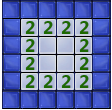
\includegraphics[scale=.5]{./demineur_1.png}
\end{figure}

Les cases bleues représentent des cases non découvertes, celles avec un chiffre ont 
été découvertes et indiquent le nombre de mines auxquelles elles touchent, soit par 
la case immédiatement au-dessus, en-dessous, à droite, à gauche ou par une des diagonales. 
Il faut donc trouver quelles cases parmi les bleues contiennent des mines. Ici, il y a 
20 cases inconnues et 12 cases qui touchent chacune à 2 mines. En résolvant cette grille, 
nous savons qu’elle contient 8 mines. Dans une approche naïve, où le joueur artificiel 
tenterait toutes les combinaisons possibles à la recherche de la meilleure 
(celle brisant le moins de contraintes) pour une grille non découverte de 6 x 6 
comme celle ci-haut (donc 36 cases), le nombre de combinaisons possibles de 8 mines serait de l’ordre de:
36!/(8!(36-8)!) = 30 260 340. 
Il faut noter que ce chiffre, bien qu’énorme, correspond au nombre de combinaisons d’une grille 
plus petite que le minimum permis dans la version Windows du jeu. \\

La résolution d’une grille de démineur peut être décomposée à la simple question de savoir quelles 
cases sont certaines (d’être minées ou non), et lesquelles sont incertaines. Un bon joueur 
artificiel de démineur ne jouera jamais une case incertaine si des cases certaines 
n’ont pas été jouées (nommées cases triviales dans nos analyses). \\

Il s’agit d’un jeu statique à agent unique partiellement observable, dans un environnement 
discret (puisqu’une grille bien délimitée est utilisée). Il s’agit aussi d’un jeu 
déterministe dans la mesure où l’action effectuée par le joueur détermine entièrement 
l’état suivant de la grille. Ce jeu est séquentiel, puisque chaque coup permet de 
découvrir une partie de la grille et restreint potentiellement le domaine des variables du prochain coup.

\section{Heuristiques et pertinence des algorithmes choisis}

Il y a plusieurs algorithmes permettant de résoudre une grille de démineur. 
Toutefois, avant de définir ceux que nous avons utilisés dans le cadre de ce travail, 
nous mentionnerons les heuristiques qui ont servi à améliorer la performance du joueur 
artificiel, puisqu’elles ont un impact sur les algorithmes :

\begin{enumerate}
        \item Frontières : notre joueur artificiel utilise les frontières pour définir 
              le domaine des cases candidates pour le prochain coup. Une frontière est 
              composée de toutes les cases entourant un indice, et a l’apparence d’un îlot 
              (voir image ci-dessous, la section violet):
                \begin{figure}[h!]
                \centering
                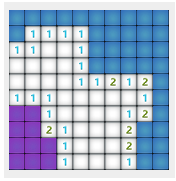
\includegraphics[scale=.5]{./demineur_2.png}
                \end{figure}
        \item Premier clic : La première case cliquée par le joueur artificiel sera 
              toujours vide (non minée et sans indice), puisqu’il n’y a aucune façon 
              d’inférer quelles cases sont minées quand il n’y en a pas une seule de 
              découverte. Notre programme construit la grille par la suite, autour de la case jouée.
        \item Backtracking avec forward checking est aussi implémenté afin d’accélérer le processus de CSP.
\end{enumerate}

En ce qui a trait aux algorithmes, le paragraphe suivant les décrit de façon non exhaustive:

\begin{enumerate}
        \item Le CSP (Constraint Satisfaction Problem) a servi comme base à tous 
              les autres algorithmes, afin d’accélérer la prise de décision en générant 
              toutes les dispositions de mines possibles (ce qui permet d’identifier les coups sûrs). 
              Les cases du jeu démineur peuvent être représentées comme des variables pouvant adopter 
              plusieurs valeurs : minée, sans mine, vide, non-découverte. Puisqu’elles sont gérées 
              par des contraintes (e.g deux cases touchant à une case ayant le chiffre 1 ne peuvent 
              pas être toutes les deux minées), CSP était tout indiqué pour être utilisé en amont aux autres algorithmes.
        \item La technique primitive du choix aléatoire (RandomArtificialPlayer) a été implémentée 
              en tout premier pour faciliter les tests et le travail sur l’interface. 
              Il s’agit simplement de choisir la prochaine case à jouer parfaitement au hasard. 
              Elle est disponible dans les choix d’algorithmes, et est utile pour des fins de comparaison/références.
        \item L’algorithme nommé “SafeOrRandomAI” dans notre programme est un simple choix 
              aléatoire sur la prochaine case à jouer, quand aucun coup sûr n’est disponible 
              (quand notre CSP n’a trouvé aucune case dont le domaine était unique).
        \item Un algorithme de raisonnement probabiliste (ProbabilisticAI) est aussi disponible. 
              Il détermine simplement la probabilité qu’une case soit minée, et utilise une 
              PriorityQueue pour stocker les coups à jouer selon leur chance d’être une 
              case vide, dans les limites des frontières établies. Lorsque toutes 
              les cases candidates ont les mêmes probabilités, il choisit au hasard la prochaine case dans sa Priority Queue.
        \item Un raisonnement probabiliste légèrement différent (nommé CrazyAI) est aussi implémenté. 
              Il tient compte de la plausibilité d’une permutation possible en lui accordant un poids. 
              Par exemple, si pour un îlot de cases voisines nous avons 4 scénarios possibles ne 
              brisant pas les contraintes, le raisonnement probabiliste précédent accorde une probabilité 
              de 25\% à chacune de ces permutations. Toutefois, pour une grille avec 
              un taux de mines de 20\%, une permutation contenant 50\% de mines, 
              par exemple, devrait être moins probable qu’un scénario contenant 20\% de 
              mines. Ainsi, un scénario avec 8 mines et 8 cases non minées, par exemple, 
              au lieu d’avoir le même poids que les autres scénarios, a un poids 
              de 0.28 x 0.88. La probabilité qu’une case individuelle ait une mine est fixe. 
              Cette contrainte vient de la séparation des frontières car elles sont évaluées 
              indépendament, ce qui fait qu’on ne peut pas prendre en compte le nombre de mines 
              trouvées dans les autres frontières. 
        \item Une autre forme de raisonnement probabiliste est utilisée, nommée “Adventurer” 
              dans notre programme. Ce raisonnement tient compte des chances qu’une case dont 
              on ne connaît pas les probabilités soit un meilleur choix que les cases dans nos frontières. 
              Par exemple, le coup suivant dévoilant un 4 nous indique qu’il y a 4 mines parmi 
              les 8 cases autour de nous (voir image suivante), ce qui signifie que nous avons une chance sur deux de 
              tomber sur une mine. Dans une grille où il resterait par exemple 4 mines à découvrir 
              sur 60 cases inconnues (donc 15\% des cases restantes étant minées), une case au 
              hasard en territoire inconnu aurait environ une chance sur 6 d’être minée, et 
              l’aventurier choisirait donc une case au hasard hors de la frontière. 
                \begin{figure}[h!]
                \centering
                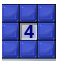
\includegraphics[scale=.5]{./demineur_3.png}
                \end{figure}
\end{enumerate}

\section{Résultats}
Pour récolter des données pour nos statistiques, nous génererons aléatoirement 5 grilles de démineur de tailles croissantes: \\
\begin{tabular}{| l | c |}
        \hline
        \textbf{Taille de la grille} & \textbf{Lignes x Colonnes} \\
        \hline
        \textbf{Petite} & 9x9 \\
        \hline
        \textbf{Moyenne} & 16x16 \\
        \hline
        \textbf{Grande} & 30x16 \\
        \hline
        \textbf{Très grande} & 100x150 \\
        \hline
        \textbf{Très très grande} & 300x400 \\
        \hline
\end{tabular}

Nous avons fixé les pourcentages suivants de mines présentes sur ces grilles: 15\%, 20\% et 25\% du nombre total de cases.

Donc, nous avons 15 scénarios possibles qui sont résolus 1000 fois par chacun des 
algorithmes mentionnés dans la section précédente. Ceci nous donne un total de 15000 
tests par algorithme et permet d’extraire les données suivantes: 

\begin{enumerate}
        \item Le nombre de victoires et défaites (Pourcentage);
        \item Le nombre de coups incertains rencontrés dans la grille (Moyenne);
        \item Le taux de réussite versus échec après incertitudes (Moyenne);
        \item Le pourcentage des “catégories” des coups joués - aléatoire, coups 
              sûrs ou aléatoire, probabiliste, probabiliste avec drapeau(prend en 
              compte le nombre de drapeaux dans les possibilités d’assignation), 
              considérer l’inconnu.
\end{enumerate}

De plus, nous comparons les temps de résolution de 10 grilles selon le nombre de 
frontières qu’elles contiennent, pour l’algorithme CSP simple, et celui avec forward-checking.
Le graphique ci-dessous démontre que l’heuristique forward-checking permet toujours de 
résoudre plus rapidement un grille de démineur que le simple CSP:

\begin{figure}[h!]
  \centering
  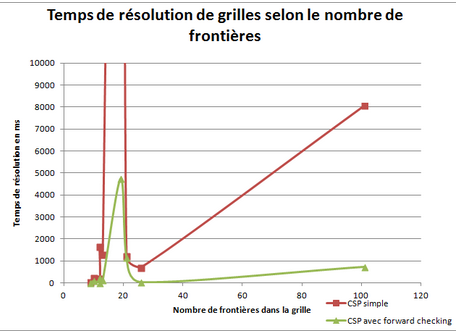
\includegraphics[scale=.5]{./vitesse.png}
\end{figure}

\section{Répartition des tâches}
\begin{enumerate}
        \item Martin: Interface et implémentation de l’algorithme CSP, avec et sans 
              MCV, ainsi que d’un joueur artificiel aléatoire pour tester 
              l’interface, heuristique du nombre de drapeaux restants.
        \item Frédéric et Louis: Raisonnements probabilistes, heuristiques pour des cases aux mêmes probabilités.
        \item Nilovna et Geneviève: Documentation (lisez-moi, rapport), présentation, 
              revampage de l’interface, mises à l’essai, statistiques, nettoyage du code et remise.
\end{enumerate}

\section{Conclusion}
Les différentes études en Intelligence Artificielle visant à résoudre le jeu de démineur proposent une panoplie d’heuristiques. Il n’y a pas de doute que ce jeu, si simple en apparence, a une compléxité intéressante. Les membres de notre équipe se sont d’ailleurs amusés à continuer à améliorer les algorithmes utilisés jusqu’à la dernière minute, si bien que nous avons manqué de temps pour les mises à l’essai. 

Cette dernière remarque nous amène à parler des améliorations possibles que nous aurions souhaité apporter à notre programme:
\begin{enumerate}
        \item Modifier la façon dont la grille est générée afin de permettre à notre programme 
              de prendre une grille en entrée, ce qui nous aurait permis d’avoir des grilles fixes 
              lors des mises à l’essai, et donc de meilleures comparaisons entre les différents algorithmes;
        \item Le calcul des probabilités dans CrazyAI pourrait tenir compte des autres cases, 
              et donc la probabilité qu’une case soit minée ne serait pas fixe;
        \item L’heuristique des coins (commencer par les cases dans les coins puisqu’elles ont 
              moins de chance d’être adjacentes à une mine et tendent à révéler des régions complètes) 
              aurait pu être implémentée afin d’améliorer la performance de notre joueur artificiel;
        \item L’heuristique MCV (Most Constrained Value) aurait pu être implémentée dans le CSP : notre joueur 
              artificiel assumerait que chaque case non-découverte est minée et l’étiqueterait d’un drapeau. 
              Par la suite, il vérifierait si les contraintes sont satisfaites. Lorsqu’il trouverait qu’une 
              contrainte est insatisfaite (car il y aurait plusieurs drapeaux consécutifs qui totaliseraient 
              plus de mines possibles que les chiffres correspondants), il utiliserait l’heuristique MCV pour retirer des drapeaux:

\begin{figure}[h!]
  \centering
  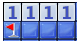
\includegraphics[scale=.5]{./demineur_4.png}
\end{figure}
La première case est assumée minée (on y pose un drapeau).

\begin{figure}[h!]
  \centering
  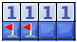
\includegraphics[scale=.5]{./demineur_5.png}
\end{figure}

La deuxième case est assumée minée (on y pose aussi un drapeau).
Contrainte violée: le premier chiffre 1 (celui à gauche) touche à deux mines. 
Il faut donc enlever la valeur “mine” à la première variable (la case à gauche).

\begin{figure}[h!]
  \centering
  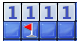
\includegraphics[scale=.5]{./demineur_6.png}
\end{figure}

Le drapeau de la première case est donc retiré, car il s’agit de la case avec le plus petit domaine de valeurs (MCV). \\

En ce qui concerne les apprentissages et les erreurs que nous avons commis lors de ce 
projet, mentionnons seulement le fait que nous avons d’abord opté pour la technique des 
réseaux bayésiens dans nos approches candidates, mais il s’est avéré qu’elle n’aurait pas
offert de meilleurs résultats que les autres algorithmes, pour beaucoup plus de travail. 

En somme, notre algorithme allie raisonnement logique et probabilisme, imitant ainsi un joueur 
humain, ce qui représente un des principaux objectifs de l'intelligence artificielle.

\end{enumerate}


\end{document}

